\documentclass[a4paper,11pt]{report}
\usepackage[T1]{fontenc}
\usepackage{fourier}
\usepackage[utf8]{inputenc}
\usepackage[french]{babel}
\usepackage{hyperref}
\usepackage{biblatex}
\usepackage{xcolor}
\usepackage[scale=0.8]{geometry}
\usepackage{graphicx}

\usepackage{listings}
\lstset{basicstyle=\ttfamily,
  showstringspaces=false,
  basicstyle=\footnotesize\ttfamily,
  keywordstyle=\bfseries\color{green!40!black},
  commentstyle=\color{purple!40!black},
  identifierstyle=\color{blue},
  stringstyle=\color{red},
  breaklines=true,
  frame=l, % single, L, lines
  framerule=2pt
}

\title{Platforme de MOOC TSP basée sur Docker}
\author{François Monniot \& Alexis Mousset}

% PDF metadata
\pdfinfo{
  /Author (François Monniot, Alexis Mousset)
  /Title (Adding PDF metadata in LaTeX)
  /Keywords (MOOC;Docker;TSP)
}

\addbibresource{report.bib}

\begin{document}

\maketitle
\tableofcontents

\begin{abstract}

\end{abstract}

\chapter{Introduction}

\section{MOOC}

\subsection{Contexte des MOOC en général}

\subsection{Contexte des MOOC à TSP}

\subsection{Contexte des besoins de TP}

\section{Docker}

\subsection{Présentation}

\subsection{Avantages et désavantages}
Pourquoi c'est bien dans notre cas, comparaison avec d'autres solution

\subsection{Comparaison avec d'autres solutions}

\chapter{Implémentation}

\section{Architecture}

La platforme que nous proposons est basé sur des conteneurs Docker. Ainsi chaque composant peut, dans l'absolu, être utilisé de manière
completement indépendante les uns des autres. La figure~\ref{architecture} représente l'architecture telle qu'envisagée lors de ce projet.

\begin{figure}[h]
   \caption{\label{architecture} Architecture de la plateforme}
   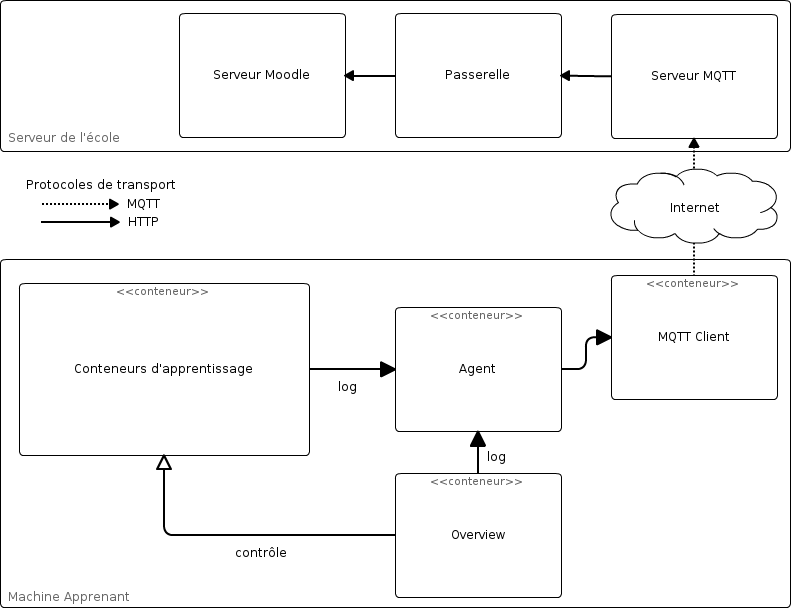
\includegraphics[width=\textwidth, keepaspectratio=true]{architecture.png}
\end{figure}

\section{Agent}

\section{Moodle}

\section{tracker.js}

\section{Overview}

\subsection{}

\subsection{}

\chapter{Utilisation}

\section{Cas d'utilisation : Le MOOC bases de données}

\subsection{Côté professeur}

L'objectif côté professeur est de faciliter la mise en place d'environnements de TP par des non spécialistes de docker (éventuellement assistés en cas de problèmes).

La configuration des machines de TP s'effectue sur un dépôt git contenant les scripts de création des environnements, ainsi que les contenus qui y seront ajoutés.

Le format de configuration est le Dockerfile, qui est constitué d'une suite de commandes lancées et de copies de fichiers. Il est très simple, si on sait configurer un système, de le consigner dans un Dockerfile.

La mise en place des TP de ce MOOC nécessite deux conteneurs : un pour la base de données et un pour le serveur et les applications web, ainsi que du conteneur permettant le suivi.

\begin{lstlisting}[language=Bash,caption={Dockerfile de base}]
RUN apt-get update && apt-get install my_software
COPY configuration_file /etc/my_software/
EXPOSE 80
# The command that should be executed
CMD ["/usr/bin/my_software"]
\end{lstlisting}


\subsection{Côté apprenant}

overview ?
plop\cite{AbedonHymanThomas2003}
\cite{website:fermentas-lambda}

\printbibliography

\end{document}
